\subsection{Styringsmodulet}
\label{sub:styringsmodul}

Styringsmodulet har til opgave at instantiere og kontrollere de moduler som udgør specifikke funktionaliteter for brugeren.

\subsubsection{Funktionalitet}
\label{ssub:hovedmodul_funktionalitet}

Når en bruger har været igennem en succesfuld validering fra loginmodulet, bliver brugeren sendt videre til styringsmodulet. Dette modul fungerer som skelettet for de omkringliggende moduler. Brugeren bevæger sig derfor hele tiden rundt indenfor dette moduls rammer, indtil brugeren ønsker at forlade programmet. Da styringsmodulet ikke selv indeholder noget information direkte til brugeren, bør den altid instantiere et default element.

\subsubsection{Implementation}
\label{ssub:hovedmodul_implementation}

\begin{figure}
  \centering
  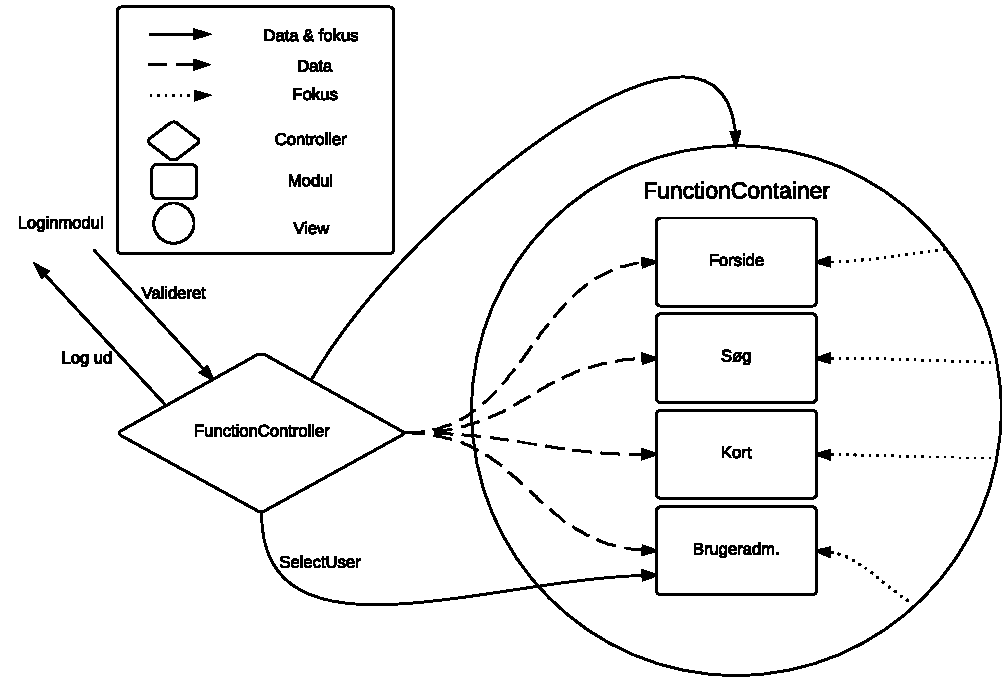
\includegraphics[width=\textwidth]{styringsmodul-diagram.pdf}
  \caption{Dette er bare noget filler tekst.}
\end{figure}


Styringsmodulet implementeres som en tabcontroller, der tilføjer andre moduler som faneblade. Default fanebladet er forsidemodulet. Dertil tilføjer styringsmodulet en kortfane, en brugerinformationsfane samt en søgningsfane. Disse faner bliver dog kun tilføjet, hvis brugeren, som er logget ind, har de nødvendige tilladelser. Når brugeren ønsker at forlade programmet, logges der ud, og brugeren sendes tilbage til loginmodulet.
